\clearpage
\begin{examplebox}
\textbf{例1（基础母题：由方程求全部四个交点）。}

\textbf{题目：}求下列两曲线的全部公共点，并说明是否共焦：
\[
E:\frac{x^2}{16}+\frac{y^2}{12}=1,
\qquad H:x^2-\frac{y^2}{3}=1.
\]
\textbf{识别信号：}椭圆、双曲线均为标准式，先算 $c$ 检验焦点是否相同。

\textbf{解：}椭圆 $a_E=4,b_E=2\sqrt3$，
$c_E=\sqrt{16-12}=2$；双曲线 $a_H=1,b_H=\sqrt3$，
$c_H=\sqrt{1+3}=2$。二者中心同为原点、焦点同为 $(\pm2,0)$。
\[
X=\frac{4\cdot1}{2}=2,\qquad
Y=\frac{(2\sqrt3)(\sqrt3)}2=3.
\]
故
\[
\boxed{(2,3),(2,-3),(-2,3),(-2,-3)}.
\]
\textbf{回代抽查：}$P=(2,3)$ 满足椭圆 $4/16+9/12=1$，
满足双曲线 $4-9/3=1$；其他三点由对称性自动满足。
\textbf{迁移：}不要只报第一象限的一个点，两个符号都要独立取正负。
\end{examplebox}

\clearpage
\begin{examplebox}
\textbf{例2（参数母题：半轴不同、点不在焦点正上方）。}

设椭圆半长轴 $a_E=5$、双曲线实半轴 $a_H=2$、
公共焦半距 $c=3$，求四个交点。

\textbf{解：}椭圆 $b_E=\sqrt{25-9}=4$；
双曲线 $b_H=\sqrt{9-4}=\sqrt5$。
故两条曲线分别为
\[
E:\frac{x^2}{25}+\frac{y^2}{16}=1,
\qquad H:\frac{x^2}{4}-\frac{y^2}{5}=1.
\]
直接代入公式得
\[
\boxed{P=\left(\pm\frac{10}{3},\ \pm\frac{4\sqrt5}{3}\right)}.
\]
\textbf{复核：}椭圆左右两项是 $4/9$ 与 $5/9$；
双曲线左右两项是 $25/9$ 与 $16/9$，差为 $1$。
\begin{center}
% Exact example 2, same x/y scale.
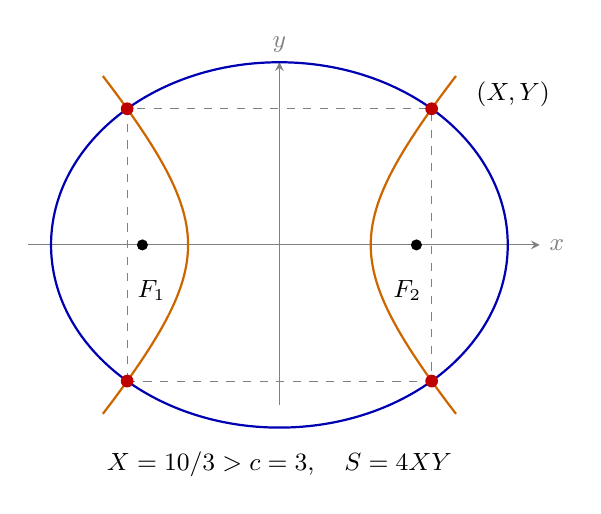
\begin{tikzpicture}[x=.58cm,y=.58cm,>=stealth,font=\small]
\draw[->,gray] (-5.5,0)--(5.7,0) node[right] {$x$};
\draw[->,gray] (0,-3.5)--(0,4) node[above] {$y$};
\draw[blue!70!black,thick] (0,0) ellipse (5 and 4);
\foreach \s in {-1,1} {
\draw[orange!80!black,thick,domain=-3.7:3.7,samples=100,variable=\t]
 plot ({\s*2*sqrt(1+\t*\t/5)},\t);}
\draw[gray,dashed] (-10/3,{-4*sqrt(5)/3}) rectangle (10/3,{4*sqrt(5)/3});
\foreach \s in {-1,1} {\foreach \t in {-1,1}
 {\fill[red!75!black] ({\s*10/3},{\t*4*sqrt(5)/3}) circle (2.3pt);}}
\fill (-3,0) circle (2pt);
\fill (3,0) circle (2pt);
\node at (-2.8,-1) {$F_1$};
\node at (2.8,-1) {$F_2$};
\node[anchor=west] at (4.1,3.3) {$(X,Y)$};
\node at (0,-4.8) {$X=10/3>c=3,\quad S=4XY$};
\end{tikzpicture}


{\small 四点构成轴平行矩形，交点横坐标大于焦半距。}
\end{center}
\textbf{图形附问：}四交点构成的矩形面积为
$4XY=4\cdot\frac{10}{3}\cdot\frac{4\sqrt5}{3}=\frac{160\sqrt5}{9}$。
\textbf{提醒：}这里 $X=10/3>c=3$，
交点不在焦点正上方；这才是一般情形。
\end{examplebox}

\clearpage
\begin{examplebox}
\textbf{例3（高考变式：只知道离心率和公共焦距）。}

共焦椭圆、双曲线的离心率分别为
$e_E=1/2$、$e_H=3/2$，公共焦半距 $c=3$。
求四个交点及两曲线的方程。

\textbf{解：}由 $a=c/e$：
\[
a_E=6,\quad a_H=2,\qquad
b_E=\sqrt{36-9}=3\sqrt3,\quad b_H=\sqrt{9-4}=\sqrt5.
\]
故
\[
E:\frac{x^2}{36}+\frac{y^2}{27}=1,\quad
H:\frac{x^2}{4}-\frac{y^2}{5}=1,
\]
\[
\boxed{P=(\pm4,\pm\sqrt{15})}.
\]
也可直接运用离心率版
\[
X=\frac{c}{e_Ee_H}=4,\qquad
Y=\frac{c\sqrt{(1-e_E^2)(e_H^2-1)}}{e_Ee_H}
=\sqrt{15}.
\]
\textbf{迁移：}只给离心率而没有 $c$ 的数值，通常只能求
$X/c$、$Y/c$ 的\emph{比例}，不能得到唯一数值坐标。
\end{examplebox}

\clearpage
\begin{examplebox}
\textbf{例4（反向构造：给定一个公共点和焦点，重建两条曲线）。}

已知共焦点 $F_1=(-2,0),F_2=(2,0)$，点 $P=(2,3)$
是某椭圆与某双曲线的共同点。求这两条标准方程，及其全部交点。

\textbf{最低门槛：}先按勾股求两条焦半径：
\[
PF_1=\sqrt{4^2+3^2}=5,\qquad PF_2=3.
\]
因椭圆\emph{和}为 $2a_E$，双曲线\emph{差}为 $2a_H$，
\[
a_E=\frac{5+3}{2}=4,\qquad a_H=\frac{5-3}{2}=1.
\]
$c=2$，所以 $b_E^2=16-4=12$、$b_H^2=4-1=3$，得
\[
\boxed{E:\frac{x^2}{16}+\frac{y^2}{12}=1},\qquad
\boxed{H:x^2-\frac{y^2}{3}=1}.
\]
四点为 $(\pm2,\pm3)$。
\textbf{迁移：}若给定 $x\ne0,y\ne0$ 的点 $P$ 和焦点 $(\pm c,0)$，
焦半径\emph{和}与\emph{绝对差}便唯一确定非退化共焦椭圆和双曲线；
若 $P$ 在 $y$ 轴上，两距离相等，只能得到 $a_H=0$ 的退化情形。
\end{examplebox}

\clearpage
\begin{examplebox}
\textbf{例5（高价值变式：无需求切线方程，证明四点处正交）。}

对例1的曲线，证明交点处两切线互相垂直，
并区分该直角与焦点三角形的角。

\textbf{解：}在 $P=(2,3)$，椭圆切线斜率
\[
k_E=-\frac{12\cdot2}{16\cdot3}=-\frac12,
\]
双曲线切线斜率
\[
k_H=\frac{3\cdot2}{1\cdot3}=2.
\]
$k_Ek_H=-1$，故两切线垂直。其余三点有
相同的斜率积；或者直接套一般的 $k_Ek_H=-1$。

与此同时，$PF_1=5,PF_2=3,F_1F_2=4$，
由余弦定理得
\[
\cos\angle F_1PF_2=\frac{5^2+3^2-4^2}{2\cdot5\cdot3}=\frac35.
\]
所以 $\angle F_1PF_2$ \textbf{不是} $90^\circ$。
\textbf{迁移：}共焦曲线的\emph{正交轨迹}属于两条\emph{切线}的性质，
焦角属于两条\emph{焦半径}的性质，这是两个不同二级结论的衔接。
\end{examplebox}
